%===============================================================================
% LaTeX sjabloon voor de bachelorproef toegepaste informatica aan HOGENT
% Meer info op https://github.com/HoGentTIN/latex-hogent-report
%===============================================================================

\documentclass[dutch,dit,thesis]{hogentreport}

% TODO:
% - If necessary, replace the option `dit`' with your own department!
%   Valid entries are dbo, dbt, dgz, dit, dlo, dog, dsa, soa
% - If you write your thesis in English (remark: only possible after getting
%   explicit approval!), remove the option "dutch," or replace with "english".

\usepackage{lipsum} % For blind text, can be removed after adding actual content

%% Pictures to include in the text can be put in the graphics/ folder
\graphicspath{{../graphics/}}

%% For source code highlighting, requires pygments to be installed
%% Compile with the -shell-escape flag!
%% \usepackage[chapter]{minted}
%% If you compile with the make_thesis.{bat,sh} script, use the following
%% import instead:
\usepackage[chapter,outputdir=../output]{minted}
\usemintedstyle{solarized-light}

%% Formatting for minted environments.
\setminted{%
    autogobble,
    frame=lines,
    breaklines,
    linenos,
    tabsize=4
}

%% Ensure the list of listings is in the table of contents
\renewcommand\listoflistingscaption{%
    \IfLanguageName{dutch}{Lijst van codefragmenten}{List of listings}
}
\renewcommand\listingscaption{%
    \IfLanguageName{dutch}{Codefragment}{Listing}
}
\renewcommand*\listoflistings{%
    \cleardoublepage\phantomsection\addcontentsline{toc}{chapter}{\listoflistingscaption}%
    \listof{listing}{\listoflistingscaption}%
}

% Other packages not already included can be imported here

%%---------- Document metadata -------------------------------------------------
% TODO: Replace this with your own information
\author{Ernst Aarden}
\supervisor{Dhr. F. Van Houte}
\cosupervisor{Mevr. S. Beeckman}
\title[Optionele ondertitel]%
    {Titel van de bachelorproef}
\academicyear{\advance\year by -1 \the\year--\advance\year by 1 \the\year}
\examperiod{1}
\degreesought{\IfLanguageName{dutch}{Professionele bachelor in de toegepaste informatica}{Bachelor of applied computer science}}
\partialthesis{false} %% To display 'in partial fulfilment'
%\institution{Internshipcompany BVBA.}

%% Add global exceptions to the hyphenation here
\hyphenation{back-slash}

%% The bibliography (style and settings are  found in hogentthesis.cls)
\addbibresource{bachproef.bib}            %% Bibliography file
\addbibresource{../voorstel/voorstel.bib} %% Bibliography research proposal
\defbibheading{bibempty}{}

%% Prevent empty pages for right-handed chapter starts in twoside mode
\renewcommand{\cleardoublepage}{\clearpage}

\renewcommand{\arraystretch}{1.2}

%% Content starts here.
\begin{document}

%---------- Front matter -------------------------------------------------------

\frontmatter

\hypersetup{pageanchor=false} %% Disable page numbering references
%% Render a Dutch outer title page if the main language is English
\IfLanguageName{english}{%
    %% If necessary, information can be changed here
    \degreesought{Professionele Bachelor toegepaste informatica}%
    \begin{otherlanguage}{dutch}%
       \maketitle%
    \end{otherlanguage}%
}{}

%% Generates title page content
\maketitle
\hypersetup{pageanchor=true}

%%=============================================================================
%% Voorwoord
%%=============================================================================

\chapter*{\IfLanguageName{dutch}{Woord vooraf}{Preface}}%
\label{ch:voorwoord}

%% TODO:
%% Het voorwoord is het enige deel van de bachelorproef waar je vanuit je
%% eigen standpunt (``ik-vorm'') mag schrijven. Je kan hier bv. motiveren
%% waarom jij het onderwerp wil bespreken.
%% Vergeet ook niet te bedanken wie je geholpen/gesteund/... heeft

\lipsum[1-2]
%%=============================================================================
%% Samenvatting
%%=============================================================================

% TODO: De "abstract" of samenvatting is een kernachtige (~ 1 blz. voor een
% thesis) synthese van het document.
%
% Een goede abstract biedt een kernachtig antwoord op volgende vragen:
%
% 1. Waarover gaat de bachelorproef?
% 2. Waarom heb je er over geschreven?
% 3. Hoe heb je het onderzoek uitgevoerd?
% 4. Wat waren de resultaten? Wat blijkt uit je onderzoek?
% 5. Wat betekenen je resultaten? Wat is de relevantie voor het werkveld?
%
% Daarom bestaat een abstract uit volgende componenten:
%
% - inleiding + kaderen thema
% - probleemstelling
% - (centrale) onderzoeksvraag
% - onderzoeksdoelstelling
% - methodologie
% - resultaten (beperk tot de belangrijkste, relevant voor de onderzoeksvraag)
% - conclusies, aanbevelingen, beperkingen
%
% LET OP! Een samenvatting is GEEN voorwoord!

%%---------- Nederlandse samenvatting -----------------------------------------
%
% TODO: Als je je bachelorproef in het Engels schrijft, moet je eerst een
% Nederlandse samenvatting invoegen. Haal daarvoor onderstaande code uit
% commentaar.
% Wie zijn bachelorproef in het Nederlands schrijft, kan dit negeren, de inhoud
% wordt niet in het document ingevoegd.

\IfLanguageName{english}{%
\selectlanguage{dutch}
\chapter*{Samenvatting}
\lipsum[1-4]
\selectlanguage{english}
}{}

%%---------- Samenvatting -----------------------------------------------------
% De samenvatting in de hoofdtaal van het document

\chapter*{\IfLanguageName{dutch}{Samenvatting}{Abstract}}

\lipsum[1-4]


%---------- Inhoud, lijst figuren, ... -----------------------------------------

\tableofcontents

% In a list of figures, the complete caption will be included. To prevent this,
% ALWAYS add a short description in the caption!
%
%  \caption[short description]{elaborate description}
%
% If you do, only the short description will be used in the list of figures

\listoffigures

% If you included tables and/or source code listings, uncomment the appropriate
% lines.
\listoftables

\listoflistings

% Als je een lijst van afkortingen of termen wil toevoegen, dan hoort die
% hier thuis. Gebruik bijvoorbeeld de ``glossaries'' package.
% https://www.overleaf.com/learn/latex/Glossaries

%---------- Kern ---------------------------------------------------------------

\mainmatter{}

% De eerste hoofdstukken van een bachelorproef zijn meestal een inleiding op
% het onderwerp, literatuurstudie en verantwoording methodologie.
% Aarzel niet om een meer beschrijvende titel aan deze hoofdstukken te geven of
% om bijvoorbeeld de inleiding en/of stand van zaken over meerdere hoofdstukken
% te verspreiden!

%%=============================================================================
%% Inleiding
%%=============================================================================

\chapter{\IfLanguageName{dutch}{Inleiding}{Introduction}}%
\label{ch:inleiding}

De inleiding moet de lezer net genoeg informatie verschaffen om het onderwerp te begrijpen en in te zien waarom de onderzoeksvraag de moeite waard is om te onderzoeken. In de inleiding ga je literatuurverwijzingen beperken, zodat de tekst vlot leesbaar blijft. Je kan de inleiding verder onderverdelen in secties als dit de tekst verduidelijkt. Zaken die aan bod kunnen komen in de inleiding~\autocite{Pollefliet2011}:

\begin{itemize}
  \item context, achtergrond
  \item afbakenen van het onderwerp
  \item verantwoording van het onderwerp, methodologie
  \item probleemstelling
  \item onderzoeksdoelstelling
  \item onderzoeksvraag
  \item \ldots
\end{itemize}

\section{\IfLanguageName{dutch}{Probleemstelling}{Problem Statement}}%
\label{sec:probleemstelling}

Uit je probleemstelling moet duidelijk zijn dat je onderzoek een meerwaarde heeft voor een concrete doelgroep. De doelgroep moet goed gedefinieerd en afgelijnd zijn. Doelgroepen als ``bedrijven,'' ``KMO's'', systeembeheerders, enz.~zijn nog te vaag. Als je een lijstje kan maken van de personen/organisaties die een meerwaarde zullen vinden in deze bachelorproef (dit is eigenlijk je steekproefkader), dan is dat een indicatie dat de doelgroep goed gedefinieerd is. Dit kan een enkel bedrijf zijn of zelfs één persoon (je co-promotor/opdrachtgever).

\section{\IfLanguageName{dutch}{Onderzoeksvraag}{Research question}}%
\label{sec:onderzoeksvraag}

Wees zo concreet mogelijk bij het formuleren van je onderzoeksvraag. Een onderzoeksvraag is trouwens iets waar nog niemand op dit moment een antwoord heeft (voor zover je kan nagaan). Het opzoeken van bestaande informatie (bv. ``welke tools bestaan er voor deze toepassing?'') is dus geen onderzoeksvraag. Je kan de onderzoeksvraag verder specifiëren in deelvragen. Bv.~als je onderzoek gaat over performantiemetingen, dan 

\section{\IfLanguageName{dutch}{Onderzoeksdoelstelling}{Research objective}}%
\label{sec:onderzoeksdoelstelling}

Wat is het beoogde resultaat van je bachelorproef? Wat zijn de criteria voor succes? Beschrijf die zo concreet mogelijk. Gaat het bv.\ om een proof-of-concept, een prototype, een verslag met aanbevelingen, een vergelijkende studie, enz.

\section{\IfLanguageName{dutch}{Opzet van deze bachelorproef}{Structure of this bachelor thesis}}%
\label{sec:opzet-bachelorproef}

% Het is gebruikelijk aan het einde van de inleiding een overzicht te
% geven van de opbouw van de rest van de tekst. Deze sectie bevat al een aanzet
% die je kan aanvullen/aanpassen in functie van je eigen tekst.

De rest van deze bachelorproef is als volgt opgebouwd:

In Hoofdstuk~\ref{ch:stand-van-zaken} wordt een overzicht gegeven van de stand van zaken binnen het onderzoeksdomein, op basis van een literatuurstudie.

In Hoofdstuk~\ref{ch:methodologie} wordt de methodologie toegelicht en worden de gebruikte onderzoekstechnieken besproken om een antwoord te kunnen formuleren op de onderzoeksvragen.

% TODO: Vul hier aan voor je eigen hoofstukken, één of twee zinnen per hoofdstuk

In Hoofdstuk~\ref{ch:conclusie}, tenslotte, wordt de conclusie gegeven en een antwoord geformuleerd op de onderzoeksvragen. Daarbij wordt ook een aanzet gegeven voor toekomstig onderzoek binnen dit domein.
\chapter{\IfLanguageName{dutch}{Stand van zaken}{State of the art}}%
\label{ch:stand-van-zaken}

% Tip: Begin elk hoofdstuk met een paragraaf inleiding die beschrijft hoe
% dit hoofdstuk past binnen het geheel van de bachelorproef. Geef in het
% bijzonder aan wat de link is met het vorige en volgende hoofdstuk.

% Pas na deze inleidende paragraaf komt de eerste sectiehoofding.

Dit hoofdstuk bevat je literatuurstudie. De inhoud gaat verder op de inleiding, maar zal het onderwerp van de bachelorproef *diepgaand* uitspitten. De bedoeling is dat de lezer na lezing van dit hoofdstuk helemaal op de hoogte is van de huidige stand van zaken (state-of-the-art) in het onderzoeksdomein. Iemand die niet vertrouwd is met het onderwerp, weet nu voldoende om de rest van het verhaal te kunnen volgen, zonder dat die er nog andere informatie moet over opzoeken \autocite{Pollefliet2011}.

Je verwijst bij elke bewering die je doet, vakterm die je introduceert, enz.\ naar je bronnen. In \LaTeX{} kan dat met het commando \texttt{$\backslash${textcite\{\}}} of \texttt{$\backslash${autocite\{\}}}. Als argument van het commando geef je de ``sleutel'' van een ``record'' in een bibliografische databank in het Bib\LaTeX{}-formaat (een tekstbestand). Als je expliciet naar de auteur verwijst in de zin (narratieve referentie), gebruik je \texttt{$\backslash${}textcite\{\}}. Soms is de auteursnaam niet expliciet een onderdeel van de zin, dan gebruik je \texttt{$\backslash${}autocite\{\}} (referentie tussen haakjes). Dit gebruik je bv.~bij een citaat, of om in het bijschrift van een overgenomen afbeelding, broncode, tabel, enz. te verwijzen naar de bron. In de volgende paragraaf een voorbeeld van elk.

\textcite{Knuth1998} schreef een van de standaardwerken over sorteer- en zoekalgoritmen. Experten zijn het erover eens dat cloud computing een interessante opportuniteit vormen, zowel voor gebruikers als voor dienstverleners op vlak van informatietechnologie~\autocite{Creeger2009}.

Let er ook op: het \texttt{cite}-commando voor de punt, dus binnen de zin. Je verwijst meteen naar een bron in de eerste zin die erop gebaseerd is, dus niet pas op het einde van een paragraaf.

\begin{figure}
  \centering
  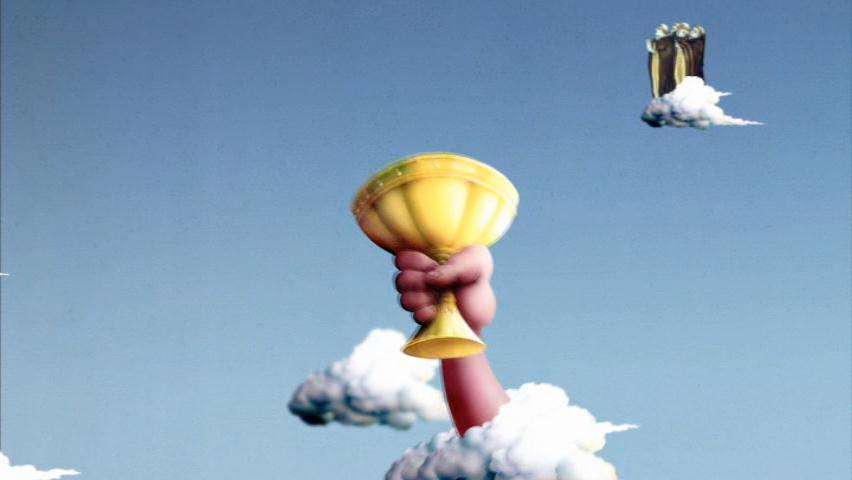
\includegraphics[width=0.8\textwidth]{grail.jpg}
  \caption[Voorbeeld figuur.]{\label{fig:grail}Voorbeeld van invoegen van een figuur. Zorg altijd voor een uitgebreid bijschrift dat de figuur volledig beschrijft zonder in de tekst te moeten gaan zoeken. Vergeet ook je bronvermelding niet!}
\end{figure}

\begin{listing}
  \begin{minted}{python}
    import pandas as pd
    import seaborn as sns

    penguins = sns.load_dataset('penguins')
    sns.relplot(data=penguins, x="flipper_length_mm", y="bill_length_mm", hue="species")
  \end{minted}
  \caption[Voorbeeld codefragment]{Voorbeeld van het invoegen van een codefragment.}
\end{listing}

\lipsum[7-20]

\begin{table}
  \centering
  \begin{tabular}{lcr}
    \toprule
    \textbf{Kolom 1} & \textbf{Kolom 2} & \textbf{Kolom 3} \\
    $\alpha$         & $\beta$          & $\gamma$         \\
    \midrule
    A                & 10.230           & a                \\
    B                & 45.678           & b                \\
    C                & 99.987           & c                \\
    \bottomrule
  \end{tabular}
  \caption[Voorbeeld tabel]{\label{tab:example}Voorbeeld van een tabel.}
\end{table}


%%=============================================================================
%% Methodologie
%%=============================================================================

\chapter{\IfLanguageName{dutch}{Methodologie}{Methodology}}%
\label{ch:methodologie}

%% TODO: In dit hoofstuk geef je een korte toelichting over hoe je te werk bent
%% gegaan. Verdeel je onderzoek in grote fasen, en licht in elke fase toe wat
%% de doelstelling was, welke deliverables daar uit gekomen zijn, en welke
%% onderzoeksmethoden je daarbij toegepast hebt. Verantwoord waarom je
%% op deze manier te werk gegaan bent.
%% 
%% Voorbeelden van zulke fasen zijn: literatuurstudie, opstellen van een
%% requirements-analyse, opstellen long-list (bij vergelijkende studie),
%% selectie van geschikte tools (bij vergelijkende studie, "short-list"),
%% opzetten testopstelling/PoC, uitvoeren testen en verzamelen
%% van resultaten, analyse van resultaten, ...
%%
%% !!!!! LET OP !!!!!
%%
%% Het is uitdrukkelijk NIET de bedoeling dat je het grootste deel van de corpus
%% van je bachelorproef in dit hoofstuk verwerkt! Dit hoofdstuk is eerder een
%% kort overzicht van je plan van aanpak.
%%
%% Maak voor elke fase (behalve het literatuuronderzoek) een NIEUW HOOFDSTUK aan
%% en geef het een gepaste titel.

\lipsum[21-25]



% Voeg hier je eigen hoofdstukken toe die de ``corpus'' van je bachelorproef
% vormen. De structuur en titels hangen af van je eigen onderzoek. Je kan bv.
% elke fase in je onderzoek in een apart hoofdstuk bespreken.

%\input{...}
%\input{...}
%...

%%=============================================================================
%% Conclusie
%%=============================================================================

\chapter{Conclusie}%
\label{ch:conclusie}

% TODO: Trek een duidelijke conclusie, in de vorm van een antwoord op de
% onderzoeksvra(a)g(en). Wat was jouw bijdrage aan het onderzoeksdomein en
% hoe biedt dit meerwaarde aan het vakgebied/doelgroep? 
% Reflecteer kritisch over het resultaat. In Engelse teksten wordt deze sectie
% ``Discussion'' genoemd. Had je deze uitkomst verwacht? Zijn er zaken die nog
% niet duidelijk zijn?
% Heeft het onderzoek geleid tot nieuwe vragen die uitnodigen tot verder 
%onderzoek?

\lipsum[76-80]



%---------- Bijlagen -----------------------------------------------------------

\appendix

\chapter{Onderzoeksvoorstel}

Het onderwerp van deze bachelorproef is gebaseerd op een onderzoeksvoorstel dat vooraf werd beoordeeld door de promotor. Dat voorstel is opgenomen in deze bijlage.

%% TODO: 
%\section*{Samenvatting}

% Kopieer en plak hier de samenvatting (abstract) van je onderzoeksvoorstel.

% Verwijzing naar het bestand met de inhoud van het onderzoeksvoorstel
%---------- Inleiding ---------------------------------------------------------

% TODO: Is dit voorstel gebaseerd op een paper van Research Methods die je
% vorig jaar hebt ingediend? Heb je daarbij eventueel samengewerkt met een
% andere student?
% Zo ja, haal dan de tekst hieronder uit commentaar en pas aan.

%\paragraph{Opmerking}

% Dit voorstel is gebaseerd op het onderzoeksvoorstel dat werd geschreven in het
% kader van het vak Research Methods dat ik (vorig/dit) academiejaar heb
% uitgewerkt (met medesturent VOORNAAM NAAM als mede-auteur).
% 

\section{Inleiding}%
\label{sec:inleiding}

In de bedrijfswereld van vandaag staat connectiviteit en beschikbaarheid centraal. Binnen deze context kan een kleine configuratiefout al snel grote gevolgen met zich mee brengen. De manuele configuratie van meerdere netwerktoestellen is een foutgevoelig en tijdrovend proces, het kan namelijk uren duren om een geheel netwerk te configureren en elke configuratielijn is een nieuwe kans op een fout.
Er is daarom nood aan een manier om het configuratieproces zowel tijdsbesparender te maken als een manier die alle toestellen consistent en foutloos kan configureren, een gepaste oplossing zou automatisatie zijn.
Dit onderzoek zal deze uitdaging proberen aanpakken door het configuratieproces te automatiseren aan de hand van Ansible. Ansible stelt ons in staat een single source of truth (SSoT) te hebben in de vorm van de Ansible controller, wat ervoor zorgt dat alle configuraties centraal beheerd, consistent toegepast en eenvoudig reproduceerbaar zijn over alle netwerktoestellen.
Naast de voordelen van een SSoT, helpt Ansible ook het hele configuratieproces te versnellen door het een, deels, hands-off proces te maken.
Deze elementen leiden naar de onderzoeksvraag \textit{in welke mate kan Ansible bijdragen aan een snellere, reproduceerbare en consistentere, schaalbare en foutloze netwerkconfiguratie binnen kmo's?}.
Het doel van deze proof-of-concept is bewijzen dat Ansible een gepaste manier is om netwerkconfiguratie sneller, consistenter, reproduceerbaar en schaalbaar te maken.
Dit onderzoek is gericht op kmo's die vaker beschikken over ICT-afdelingen met een beperkt aantal netwerkbeheerders die vaak beperkt zijn in hun tijd om een geheel netwerk, toestel per toestel, te (her)configureren.

%---------- Stand van zaken ---------------------------------------------------

\section{Literatuurstudie}%
\label{sec:literatuurstudie}

ICT de ruggengraat van het bedrijfsleven noemen is geen toekomstvisie meer, maar de hedendaagse realiteit \autocite{OlalereAbiodun2023}. 
Zo goed als elke organisatie vertrouwt op digitale infrastructuur om hun communicatie en dienstverlening efficiënt te laten verlopen.
Een netwerk dat 24/7 beschikbaar is staat hierin centraal, maar wat als er tijdens de configuratie van het netwerk een fout wordt gemaakt die ervoor zorgt dat cruciale diensten offline worden gehaald?
Om bedrijfscontinuïteit te garanderen is er dus nood aan een manier om het netwerk consistent en foutloos te kunnen configureren.
Waarom automatiseren? Netwerken zijn doorheen de jaren een stuk complexer geworden. Waar vroeger een kleine hoeveelheid toestellen lokaal beheerd werden, beschikken organisaties vandaag over tientallen of honderden netwerktoestellen op verschillende locaties. 
Tientallen toestellen manueel configureren is niet alleen een tijdrovend proces, een reeks netwerktoestellen productieklaar maken kan al snel uren duren en het proces automatiseren kan dit verkorten naar slechts enkele minuten \autocite{Younes2024}.
Naast de tijd die verloren wordt bij manuele configuratie is er nog een groot probleem: elke configuratielijn is een nieuwe kans op een menselijke fout. 
Automatisatie is een mogelijke oplossing die al getoond heeft dat het aantal menselijke fouten die gemaakt worden aanzienlijk daalt \autocite{Diekmann_2015}.
Hoewel de voordelen van automatisatie duidelijk en gekend zijn, blijven organisaties vaak vasthouden aan manuele configuratie. 
De terughoudendheid van organisaties ligt voornamelijk bij een gebrek aan kennis over automatisatietools, angst voor verandering of de investering in tijd en middelen die nodig is om automatisatie te implementeren \autocite{EMAItential2021}.
Een mogelijke manier om deze zorgen te overbruggen is een gebruiksvriendelijke, goed ondersteunde automatisatietool: Ansible.
Ansible is een open-source automatisatietool, ontwikkeld door Red Hat, die gebruik maakt van een agentless architectuur.
Dit betekent dat er geen aparte software op de netwerktoestellen hoeft te worden geïnstalleerd aangezien Ansible rechtstreeks met de netwerkapparatuur communiceert aan de hand van SSH of API's. Configuraties worden beschreven in eenvoudige YAML-bestanden, playbooks, waarin de gewenste toestand van het netwerk wordt gedefinieerd.
Deze declaratieve aanpak maakt het mogelijk om complexe configuraties herhaalbaar, consistent en foutloos uit te voeren, waarbij de Ansible controller (een server of computer vanwaar alle Ansible-taken worden uitgevoerd en beheerd) met alle configuratiebestanden fungeert als een single source of truth (SSoT).
Ansible biedt ook ondersteuning voor een breed assortiment aan netwerkapparatuur, waaronder Cisco, waarop dit onderzoek zich gaat focussen, via Ansible Collections.
Hierdoor kunnen kmo's hun bestaande infrastructuur automatiseren zonder afhankelijk te zijn van één specifieke leverancier, wat bijdraagt aan flexibiliteit en schaalbaarheid \autocite{Cisco2022}.
Naast de eerder genoemde voordelen biedt Ansible ook uitgebreide documentatie en een actieve community, wat het leerproces en de implementatie vergemakkelijkt alsook ondersteuning biedt bij implementatieproblemen.
Dit onderzoek zal ingaan op hoe Ansible gebruikt kan worden in de configuratie van een netwerk binnen kmo's om menselijke fouten te verminderen, het configuratieproces te versnellen en de consistentie, reproduceerbaarheid en schaalbaarheid te vergroten.

%---------- Methodologie ------------------------------------------------------
\section{Methodologie}%
\label{sec:methodologie}

Om de proof-of-concept te realiseren, wordt een kwantitatieve en experimentele onderzoeksmethode toegepast. Deze methodologie bestaat uit vier hoofdfasen: voorbereiding, ontwerp, implementatie en evaluatie.

\subsection{Voorbereidingsfase}
In de voorbereidingsfase wordt de bestaande netwerkarchitectuur van een typische kmo bestudeerd om een realistische testomgeving te kunnen opzetten. Het einddoel van deze fase is het volgende in kaart brengen:
\begin{itemize}
  \item Welke netwerktoestellen (zoals switches en routers) zullen gebruikt worden.
  \item Welke configuratieparameters representatief zijn voor een netwerktoestel binnen een kmo (zoals VLAN's, IP-adressering en routing).
  \item Welke handelingen netwerkbeheerders typisch manueel uitvoeren.
\end{itemize}
Op basis van deze analyse wordt een representatieve testomgeving uitgewerkt die de netwerkstructuur van een kmo nabootst. Dit gebeurt in een virtuele omgeving om risico's op productieomgevingen te vermijden.

\subsection{Ontwerpfase}
In deze fase wordt het automatisatieconcept ontworpen aan de hand van Ansible. Hierbij worden:
\begin{itemize}
  \item Een Ansible controller opgezet als centraal beheerpunt.
  \item Playbooks opgesteld die de gewenste netwerkconfiguratie beschrijven in YAML-formaat.
  \item Inventarissen aangemaakt die de netwerktoestellen definiëren en groeperen.
\end{itemize}
Daarnaast wordt het concept van een single source of truth (SSoT) geïntegreerd door alle configuratiebestanden centraal te beheren op de controller. Dit ontwerp garandeert consistentie en herhaalbaarheid over alle toestellen.

\subsection{Implementatiefase}
De implementatiefase richt zich op het toepassen en testen van de Ansible-configuraties. De volgende stappen worden uitgevoerd:
\begin{enumerate}
  \item Configuratie van virtuele netwerktoestellen (Cisco IOS in GNS3).
  \item Verbinding tussen de Ansible controller en de netwerktoestellen via SSH.
  \item Uitvoering van playbooks voor basisconfiguratie (hostname, interfaces, VLAN's, routing, etc).
  \item Herhaalde uitvoering van dezelfde playbooks om de reproduceerbaarheid te testen.
\end{enumerate}
Tijdens deze fase wordt gemeten hoeveel tijd nodig is voor configuratie met en zonder automatisatie, en wordt het aantal fouten geregistreerd om de impact van automatisatie te evalueren.

\subsection{Evaluatiefase}
Tot slot wordt het proof-of-concept geëvalueerd op basis van meetbare criteria:
\begin{itemize}
  \item \textbf{Tijdswinst}: vergelijking van manuele versus geautomatiseerde configuratie.
  \item \textbf{Reproduceerbaarheid en Consistentie}: mogelijkheid om dezelfde configuratie meerdere keren zonder afwijkingen toe te passen.
  \item \textbf{Schaalbaarheid}: evaluatie van de prestaties bij meerdere netwerktoestellen.
  \item \textbf{Foutvermindering}: Worden er minder fouten gemaakt bij een configuratie met behulp van Ansible.

\end{itemize}
De resultaten van deze evaluatie dienen om te bepalen of Ansible effectief een haalbare en efficiënte oplossing biedt voor netwerkconfiguratie binnen kmo's.

\subsection{Tools en technologieën}
Voor dit onderzoek worden de volgende tools en technologieën gebruikt:
\begin{itemize}
  \item \textbf{Ansible}: automatisatietool voor configuratiebeheer.
  \item \textbf{Cisco IOS} (virtueel): voor representatieve netwerktoestellen.
  \item \textbf{GNS3}: simulatieplatform voor netwerkarchitecturen.
  \item \textbf{Python en YAML}: voor het schrijven en aanpassen van playbooks.
\end{itemize}
Deze combinatie van technologieën maakt het mogelijk om het volledige configuratieproces gecontroleerd, herhaalbaar en meetbaar uit te voeren.


%---------- Verwachte resultaten ----------------------------------------------
\section{Verwacht resultaat, conclusie}%
\label{sec:verwachte_resultaten}

Het doel van dit onderzoek is om aan te tonen dat netwerkconfiguratie automatiseren met Ansible leidt tot een snellere, consistentere en meer schaalbare manier van configureren waarbij minder fouten worden gemaakt in vergelijking met traditionele, manuele configuratie.
De verwachte resultaten worden opgesplitst in vier categorieën: tijdswinst, reproduceerbaarheid en consistentie, schaalbaarheid en foutvermindering.

\subsection{Tijdswinst}

Ansible playbooks stellen netwerkbeheerders in staat de configuratietijd aanzienlijk te verminderen.
Een netwerk configureren op de traditionele manier houdt in dat de netwerkbeheerder elk commando op elk toestel manueel moet invoeren, Ansible daarentegen voert de configuratie parallel uit op alle toestellen.
Door de configuratie parallel uit te voeren wordt er een tijdwinst van 60-80\% verwacht, afhankelijk van de grootte van het netwerk en de complexiteit van de configuratie.
De grootste tijdswinst zal echter te vinden zijn bij herconfiguratie of aanpassingen, doordat alles centraal beheerd wordt in de inventaris van de controller. 
Aangezien de configuratie, zoals eerder vernoemd, parallel verloopt en op basis van de controller als SSoT, moet een wijziging in adressering, routing of VLAN's niet handmatig op elk toestel worden uitgevoerd.
De netwerkbeheerder moet enkel de gewenste aanpassing doorvoeren in playbooks en inventarisbestanden en de playbooks uitvoeren.
Ansible zorgt er vervolgens voor dat deze wijziging automatisch en consistent wordt toegepast op alle relevante toestellen.

\subsection{Reproduceerbaarheid en Consistentie}

Netwerkconfiguratie consistent houden is nog een voordeel dat Ansible met zich meebrengt. 
De declaratieve aanpak houdt in dat alle toestellen en configuraties in inventarisbestanden en playbooks worden verwerkt.
Deze aanpak brengt het voordeel van consistentie met zich mee aangezien alles op dezelfde manier wordt geconfigureerd.
Ook worden configuraties die afhankelijk zijn van verwijzingen altijd meegenomen vanuit de inventarisbestanden en playbooks.
Deze voordelen zijn vooral merkbaar bij aanpassingen of uitbreidingen van het netwerk.  
Zo kan bijvoorbeeld een routingtabel eenvoudig worden aangepast of aangevuld op basis van de inventaris, zonder dat er nog verwijzingen bestaan naar servers die een nieuw IP-adres hebben gekregen 
of hoeft bij de toevoeging van een nieuwe router niet langer op elke bestaande router handmatig een extra route worden geconfigureerd — Ansible past de wijziging automatisch toe op alle relevante toestellen.

\subsection{Schaalbaarheid}
Naarmate het aantal netwerktoestellen toeneemt, blijft de uitvoeringstijd grotendeels constant, aangezien de configuratie parallel kan worden uitgerold.  
Het verwachte resultaat is dat de complexiteit van het netwerk slechts een beperkte invloed heeft op de configuratietijd, wat aantoont dat de oplossing schaalbaar is naar grotere bedrijfsnetwerken.

\subsection{Foutvermindering}
Omdat alle configuraties in één centraal beheerd bestand (de Ansible controller) worden opgeslagen en uitgerold, wordt verwacht dat het aantal menselijke fouten sterk afneemt.  
Configuraties die met Ansible worden uitgerold zijn bovendien herhaalbaar en identiek, wat menselijke typfouten of inconsistenties uitsluit.  
Het verwachte resultaat is een daling van het aantal configuratiefouten tot nagenoeg nul, aangezien elke wijziging via hetzelfde playbook wordt toegepast op alle toestellen.

\subsection{Conclusie}
Ansible is een makkelijke en goedkope manier om netwerkconfiguratie sneller, reproduceerbaar, consistenter en meer schaalbaar te maken, alsook het aantal fouten dat gemaakt wordt bij de configuratie drastisch te verminderen.
Het is een mature technologie met veel documentatie en een grote community wat ervoor zorgt dat het schrijven van playbooks en de implementatie ervan een laagdrempelige stap naar automatisatie is.


%%---------- Andere bijlagen --------------------------------------------------
% TODO: Voeg hier eventuele andere bijlagen toe. Bv. als je deze BP voor de
% tweede keer indient, een overzicht van de verbeteringen t.o.v. het origineel.
%\input{...}

%%---------- Backmatter, referentielijst ---------------------------------------

\backmatter{}

\setlength\bibitemsep{2pt} %% Add Some space between the bibliograpy entries
\printbibliography[heading=bibintoc]

\end{document}
